\documentclass[11pt,a4paper]{report}
\usepackage[textwidth=37em,vmargin=30mm]{geometry}
\usepackage{calc,xunicode,amsmath,amssymb,paralist,enumitem,tabu,booktabs,datetime2,xeCJK,xeCJKfntef,listings}
\usepackage{tocloft,fancyhdr,tcolorbox,xcolor,graphicx,eso-pic,xltxtra,xelatexemoji}

\newcommand{\envyear}[0]{2025}
\newcommand{\envdatestr}[0]{2025-03-11}
\newcommand{\envfinaldir}[0]{webdb/2025/20250311/final}

\usepackage[hidelinks]{hyperref}
\hypersetup{
    colorlinks=false,
    pdfpagemode=FullScreen,
    pdftitle={Web Digest - \envdatestr}
}

\setlength{\cftbeforechapskip}{10pt}
\renewcommand{\cftchapfont}{\rmfamily\bfseries\large\raggedright}
\setlength{\cftbeforesecskip}{2pt}
\renewcommand{\cftsecfont}{\sffamily\small\raggedright}

\setdefaultleftmargin{2em}{2em}{1em}{1em}{1em}{1em}

\usepackage{xeCJK,xeCJKfntef}
\xeCJKsetup{PunctStyle=plain,RubberPunctSkip=false,CJKglue=\strut\hskip 0pt plus 0.1em minus 0.05em,CJKecglue=\strut\hskip 0.22em plus 0.2em}
\XeTeXlinebreaklocale "zh"
\XeTeXlinebreakskip = 0pt


\setmainfont{Brygada 1918}
\setromanfont{Brygada 1918}
\setsansfont{IBM Plex Sans}
\setmonofont{JetBrains Mono NL}
\setCJKmainfont{Noto Serif CJK SC}
\setCJKromanfont{Noto Serif CJK SC}
\setCJKsansfont{Noto Sans CJK SC}
\setCJKmonofont{Noto Sans CJK SC}

\setlength{\parindent}{0pt}
\setlength{\parskip}{8pt}
\linespread{1.15}

\lstset{
	basicstyle=\ttfamily\footnotesize,
	numbersep=5pt,
	backgroundcolor=\color{black!5},
	showspaces=false,
	showstringspaces=false,
	showtabs=false,
	tabsize=2,
	captionpos=b,
	breaklines=true,
	breakatwhitespace=true,
	breakautoindent=true,
	linewidth=\textwidth
}






\newcommand{\coverpic}[2]{
    % argv: itemurl, authorname
    Cover photo by #2~~(\href{#1}{#1})
}
\newcommand{\makeheader}[0]{
    \begin{titlepage}
        % \newgeometry{hmargin=15mm,tmargin=21mm,bmargin=12mm}
        \begin{center}
            
            \rmfamily\scshape
            \fontspec{BaskervilleF}
            \fontspec{Old Standard}
            \fontsize{59pt}{70pt}\selectfont
            WEB\hfill DIGEST
            
            \vfill
            % \vskip 30pt
            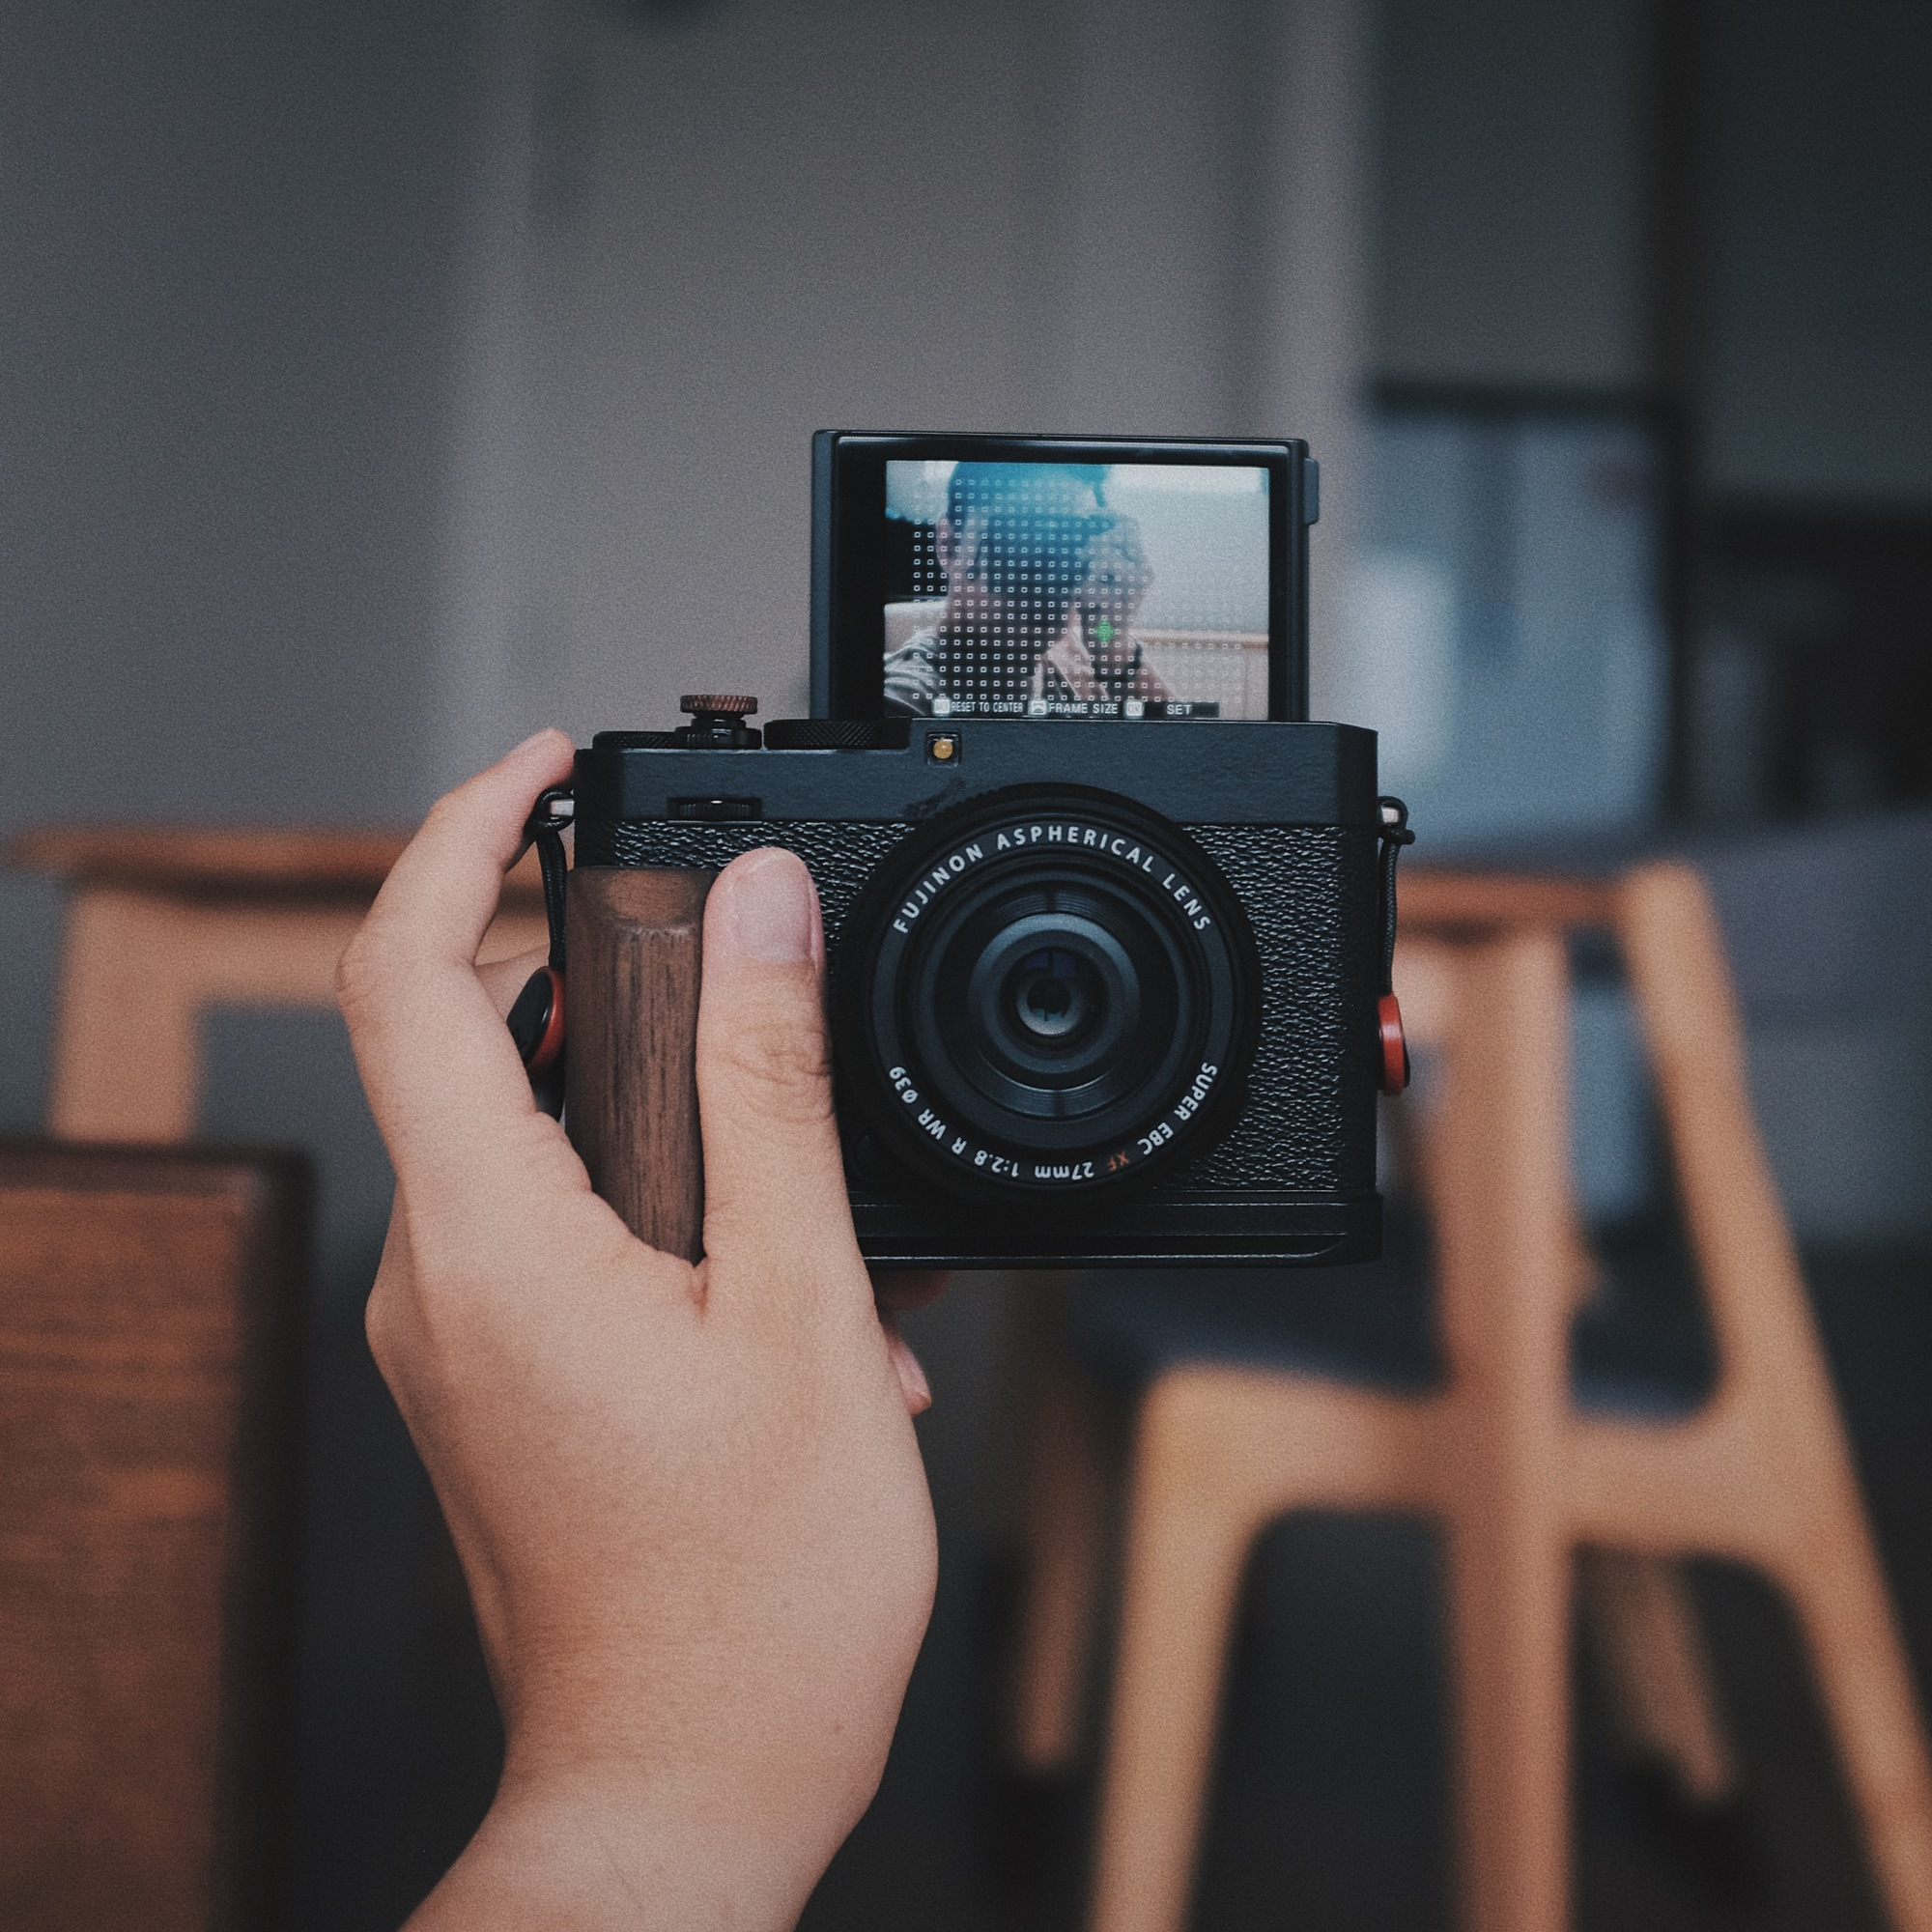
\includegraphics[width=\linewidth]{\envfinaldir/coverpic-prod.jpg}\par
            % \vskip 30pt
            \vfill

            \normalsize\rmfamily\scshape
            \copyright{} The Web Digest Project \hfill\large \envdatestr
        \end{center}
    \end{titlepage}
    % \restoregeometry
}
\newcommand{\simplehref}[1]{%
    \textcolor{blue!80!green}{\href{#1}{#1}}%
}
\renewcommand{\contentsname}{\center\Huge\sffamily\bfseries Contents\par\vskip 20pt}
\newcounter{ipartcounter}
\setcounter{ipartcounter}{0}
\newcommand{\ipart}[1]{
    % \vskip 20pt
    \clearpage
    \stepcounter{ipartcounter}
    \phantomsection
    \addcontentsline{toc}{chapter}{#1}
    % \begin{center}
    %     \Huge
    %     \sffamily\bfseries
    %     #1
    % \end{center}
    % \vskip 20pt plus 7pt
}
\newcounter{ichaptercounter}
\setcounter{ichaptercounter}{0}
\newcommand{\ichapter}[1]{
    % \vskip 20pt
    \clearpage
    \stepcounter{ichaptercounter}
    \phantomsection
    \addcontentsline{toc}{section}{\numberline{\arabic{ichaptercounter}}#1}
    \begin{center}
        \Huge
        \sffamily\bfseries
        #1
    \end{center}
    \vskip 20pt plus 7pt
}
\newcommand{\entrytitlefont}[1]{\subsection*{\raggedright\Large\sffamily\bfseries#1}}
\newcommand{\entryitemGeneric}[2]{
    % argv: title, url
    \parbox{\linewidth}{
        \entrytitlefont{#1}\par\vskip 5pt
        \footnotesize\ttfamily\mdseries
        \simplehref{#2}
    }\vskip 11pt plus 11pt minus 1pt
}
\newcommand{\entryitemGithub}[3]{
    % argv: title, url, desc
    \parbox{\linewidth}{
        \entrytitlefont{#1}\par\vskip 5pt
        \footnotesize\ttfamily\mdseries
        \simplehref{#2}\par\vskip 5pt
        \small\rmfamily\mdseries#3
    }\vskip 11pt plus 11pt minus 1pt
}
\newcommand{\entryitemAp}[3]{
    % argv: title, url, desc
    \parbox{\linewidth}{
        \entrytitlefont{#1}\par\vskip 5pt
        \footnotesize\ttfamily\mdseries
        \simplehref{#2}\par\vskip 5pt
        \small\rmfamily\mdseries#3
    }\vskip 11pt plus 11pt minus 1pt
}
\newcommand{\entryitemHackernews}[3]{
    % argv: title, hnurl, rawurl
    % \parbox{\linewidth}{
    %     \entrytitlefont{#1}\par\vskip 5pt
    %     \footnotesize\ttfamily\mdseries
    %     \simplehref{#3}\par
    %     \textcolor{black!50}{\href{#2}{#2}}
    % }\vskip 11pt plus 11pt minus 1pt
    \begin{minipage}{\linewidth}
            \entrytitlefont{#1}\par\vskip 5pt
            \footnotesize\ttfamily\mdseries
            \simplehref{#3}\par
            \textcolor{black!50}{\href{#2}{#2}}
    \end{minipage}\par\vskip 11pt plus 11pt minus 1pt
}







\begin{document}

\makeheader

\tableofcontents\clearpage




\ipart{Developers}
\ichapter{Hacker News}
\entryitemTwoLinks{British tourist detained by US authorities for 10 days over visa issue}{https://news.ycombinator.com/item?id=43324040}{https://www.theguardian.com/uk-news/2025/mar/10/british-tourist-detained-us-authorities-10-days-visa-issue}

\entryitemTwoLinks{Mathematical Foundations of Reinforcement Learning}{https://news.ycombinator.com/item?id=43323946}{https://github.com/MathFoundationRL/Book-Mathematical-Foundation-of-Reinforcement-Learning}

\entryitemTwoLinks{Firmware update bricks HP printers, makes them unable to use HP cartridges}{https://news.ycombinator.com/item?id=43323923}{https://arstechnica.com/gadgets/2025/03/firmware-update-bricks-hp-printers-makes-them-unable-to-use-hp-cartridges/}

\entryitemTwoLinks{People are just as bad as my LLMs}{https://news.ycombinator.com/item?id=43323755}{https://wilsoniumite.com/2025/03/10/people-are-just-as-bad-as-my-llms/}

\entryitemTwoLinks{Wall Street sell-off turns 'ugly' as US recession fears grow}{https://news.ycombinator.com/item?id=43323652}{https://www.independent.co.uk/business/wall-street-selloff-turns-ugly-as-us-recession-fears-grow-b2712420.html}

\entryitemTwoLinks{Washington Post editor resigns after accusing CEO of killing column}{https://news.ycombinator.com/item?id=43323519}{https://www.nbcnews.com/news/us-news/washington-post-editor-ruth-marcus-resigns-accusing-ceo-killing-column-rcna195634}

\entryitemTwoLinks{DOJ: Google must sell Chrome, Android could be next}{https://news.ycombinator.com/item?id=43323485}{https://arstechnica.com/google/2025/03/doj-google-must-sell-chrome-android-could-be-next/}

\entryitemTwoLinks{Software-Defined Radio for Engineers (2018) [pdf]}{https://news.ycombinator.com/item?id=43323071}{https://www.analog.com/media/en/training-seminars/design-handbooks/Software-Defined-Radio-for-Engineers-2018/SDR4Engineers.pdf}

\entryitemTwoLinks{uBlock Origin is no longer available on the Chrome Store}{https://news.ycombinator.com/item?id=43322922}{https://chromewebstore.google.com/detail/ublock-origin/cjpalhdlnbpafiamejdnhcphjbkeiagm?hl=en}

\entryitemTwoLinks{Wall Street stocks tumble as investors fret over US economic slowdown}{https://news.ycombinator.com/item?id=43322776}{https://www.ft.com/content/7f836a84-4fa5-4cd9-bcca-4e98d5a2e2a4}

\entryitemTwoLinks{Music labels will regret coming for the Internet Archive, sound historian says}{https://news.ycombinator.com/item?id=43322245}{https://arstechnica.com/tech-policy/2025/03/music-labels-will-regret-coming-for-the-internet-archive-sound-historian-says/}

\entryitemTwoLinks{Show HN: Editable Games}{https://news.ycombinator.com/item?id=43321688}{https://playscl.com/make}

\entryitemTwoLinks{YouTube DRM added on ALL videos with TV (TVHTML5) clients}{https://news.ycombinator.com/item?id=43321145}{https://github.com/yt-dlp/yt-dlp/issues/12563}

\entryitemTwoLinks{Canon EF and RF Lenses – All Autofocus Motors}{https://news.ycombinator.com/item?id=43320230}{https://exclusivearchitecture.com/03-technical-articles-CLT-12-autofocus-systems.html}

\entryitemTwoLinks{Real Chilling Effects}{https://news.ycombinator.com/item?id=43318842}{https://donmoynihan.substack.com/p/real-chilling-effects}

\entryitemTwoLinks{Go European: Discover European products and services}{https://news.ycombinator.com/item?id=43318798}{https://www.goeuropean.org/}

\entryitemTwoLinks{European Cloud Computing Platforms}{https://news.ycombinator.com/item?id=43318738}{https://european-alternatives.eu/category/cloud-computing-platforms}

\entryitemTwoLinks{Probabilistic Artificial Intelligence}{https://news.ycombinator.com/item?id=43318624}{https://arxiv.org/abs/2502.05244}

\entryitemTwoLinks{Trees not profits: we're giving up our right to ever sell Ecosia (2018)}{https://news.ycombinator.com/item?id=43317887}{https://blog.ecosia.org/trees-not-profits/}

\entryitemTwoLinks{Contra Chrome: How Google's browser became a threat to privacy and democracy}{https://news.ycombinator.com/item?id=43317677}{https://contrachrome.com}\ichapter{Phoronix}
\entryitemGeneric{\hskip 0pt{}OpenZFS 2.3.1 Released With Linux 6.13 Compatibility, Many Fixes}{https://www.phoronix.com/news/OpenZFS-2.3.1-Released}

\entryitemGeneric{\hskip 0pt{}Mir 2.20 Brings Focus Stealing Prevention, Workaround/Quirk Fixes}{https://www.phoronix.com/news/Mir-2.20-Released}

\entryitemGeneric{\hskip 0pt{}Box64 0.3.4 Released: Faster \& Steam Now Runs With Box32 On ARM64}{https://www.phoronix.com/news/Box64-0.3.4-Released}

\entryitemGeneric{\hskip 0pt{}DRM User-Space API For Apple Silicon Graphics Posted For Review}{https://www.phoronix.com/news/DRM-User-Space-API-Asahi}

\entryitemGeneric{\hskip 0pt{}AMD EPYC 9845 Makes For A Persuasive Upgrade With Performance \& Energy Efficiency}{https://www.phoronix.com/review/amd-epyc-9845}

\entryitemGeneric{\hskip 0pt{}Fedora 43 Looking At RPM 6.0, JPEG-XL Wallpapers \& Other Early Change Proposals}{https://www.phoronix.com/news/Fedora-43-RPM-6.0-Early-Changes}

\entryitemGeneric{\hskip 0pt{}ASUS PRIME X670E-PRO WIFI \& AMD BC-250 Sensor Monitoring With Linux 6.15}{https://www.phoronix.com/news/Linux-6.15-Early-HWMON}

\entryitemGeneric{\hskip 0pt{}Intel Preps Xe3's "Dirty Rect" Feature For Linux 6.15}{https://www.phoronix.com/news/Intel-Xe3-Dirty-Rect-Linux-6.15}

\entryitemGeneric{\hskip 0pt{}Linux's ARM Apple Support Now Has Another Code Reviewer}{https://www.phoronix.com/news/Apple-Linux-Another-Reviewer}\ichapter{Dribbble}
\entryitemGeneric{\hskip 0pt{}Crystal // Website}{https://dribbble.com/shots/25742820-Crystal-Website}

\entryitemGeneric{\hskip 0pt{}OneC1 - Logo Design}{https://dribbble.com/shots/25732400-OneC1-Logo-Design}

\entryitemGeneric{\hskip 0pt{}Ecommerce illustration}{https://dribbble.com/shots/25734258-Ecommerce-illustration}

\entryitemGeneric{\hskip 0pt{}Best Friends}{https://dribbble.com/shots/25730832-Best-Friends}

\entryitemGeneric{\hskip 0pt{}Free Fly Apparel}{https://dribbble.com/shots/25727838-Free-Fly-Apparel}

\entryitemGeneric{\hskip 0pt{}Columbus Rapids® C-Wave}{https://dribbble.com/shots/25727535-Columbus-Rapids-C-Wave}

\entryitemGeneric{\hskip 0pt{}Bloodhound Detective}{https://dribbble.com/shots/25726401-Bloodhound-Detective}

\entryitemGeneric{\hskip 0pt{}QLOUD - Logo Redesign}{https://dribbble.com/shots/25726630-QLOUD-Logo-Redesign}

\entryitemGeneric{\hskip 0pt{}Faithful web design}{https://dribbble.com/shots/25723024-Faithful-web-design}

\entryitemGeneric{\hskip 0pt{}Dj Dule logo}{https://dribbble.com/shots/25725864-Dj-Dule-logo}

\entryitemGeneric{\hskip 0pt{}Puzzle Fintech Website Design}{https://dribbble.com/shots/25651990-Puzzle-Fintech-Website-Design}

\entryitemGeneric{\hskip 0pt{}Dashboard for an Education Product ✦ Golf Pro}{https://dribbble.com/shots/25720487-Dashboard-for-an-Education-Product-Golf-Pro}

\entryitemGeneric{\hskip 0pt{}Proboscis Monkey}{https://dribbble.com/shots/25720978-Proboscis-Monkey}

\entryitemGeneric{\hskip 0pt{}Logofolio Update - March 2025}{https://dribbble.com/shots/25719985-Logofolio-Update-March-2025}

\entryitemGeneric{\hskip 0pt{}FUUL // Branding Identity}{https://dribbble.com/shots/25719928-FUUL-Branding-Identity}

\entryitemGeneric{\hskip 0pt{}Bento grid barbershop platform UI}{https://dribbble.com/shots/25715947-Bento-grid-barbershop-platform-UI}

\entryitemGeneric{\hskip 0pt{}Cimet Slogan}{https://dribbble.com/shots/25710581-Cimet-Slogan}

\entryitemGeneric{\hskip 0pt{}Brickken UX/UI design}{https://dribbble.com/shots/25721894-Brickken-UX-UI-design}

\entryitemGeneric{\hskip 0pt{}Letter C + Hummingbird}{https://dribbble.com/shots/25713900-Letter-C-Hummingbird}

\entryitemGeneric{\hskip 0pt{}Real Estate Platform UI}{https://dribbble.com/shots/25711538-Real-Estate-Platform-UI}

\entryitemGeneric{\hskip 0pt{}Logistics Company Web Design Landing Page}{https://dribbble.com/shots/25708252-Logistics-Company-Web-Design-Landing-Page}

\entryitemGeneric{\hskip 0pt{}Easy A Deck}{https://dribbble.com/shots/25715917-Easy-A-Deck}

\entryitemGeneric{\hskip 0pt{}Landing Page: AI Testing}{https://dribbble.com/shots/25714074-Landing-Page-AI-Testing}

\entryitemGeneric{\hskip 0pt{}Inner Truth}{https://dribbble.com/shots/25659901-Inner-Truth}


\ipart{Developers~~~~(zh-Hans)}
\ichapter{Solidot}
\entryitemGeneric{\hskip 0pt{}欧洲开发 RISC-V 超算}{https://www.solidot.org/story?sid=80748}

\entryitemGeneric{\hskip 0pt{}吃超加工食品会伤害你的肠道}{https://www.solidot.org/story?sid=80747}

\entryitemGeneric{\hskip 0pt{}中国男子因运营日本盗版动漫网站被捕}{https://www.solidot.org/story?sid=80746}

\entryitemGeneric{\hskip 0pt{}小鼠会给同伴做急救}{https://www.solidot.org/story?sid=80745}

\entryitemGeneric{\hskip 0pt{}广泛使用的蓝牙芯片包含未公开的隐藏命令,能被本地利用}{https://www.solidot.org/story?sid=80744}

\entryitemGeneric{\hskip 0pt{}四成英国人过去 12 个月没有读过一本书}{https://www.solidot.org/story?sid=80743}

\entryitemGeneric{\hskip 0pt{}Google 推出 Debian Linux Terminal App For Android }{https://www.solidot.org/story?sid=80742}

\entryitemGeneric{\hskip 0pt{}美国司法部仍然想要 Google 出售 Chrome }{https://www.solidot.org/story?sid=80741}

\entryitemGeneric{\hskip 0pt{}美国的蝴蝶数量过去二十年减少了 22\%}{https://www.solidot.org/story?sid=80740}

\entryitemGeneric{\hskip 0pt{}Reddit 的 AutoModerator 系统将 Luigi 标记为潜在暴力内容}{https://www.solidot.org/story?sid=80739}

\entryitemGeneric{\hskip 0pt{}印度女性每天在无偿家务上的时间两倍多于男性}{https://www.solidot.org/story?sid=80738}

\entryitemGeneric{\hskip 0pt{}巴西法官命令苹果在 90 天内开放其 iOS 平台}{https://www.solidot.org/story?sid=80737}

\entryitemGeneric{\hskip 0pt{}微软开发与 OpenAI 竞争的大模型 MAI}{https://www.solidot.org/story?sid=80736}

\entryitemGeneric{\hskip 0pt{}柯伊伯带可能有很多三体系统}{https://www.solidot.org/story?sid=80735}

\entryitemGeneric{\hskip 0pt{}Intuitive Machines 的雅典娜月球探测器因侧翻而提前终止任务}{https://www.solidot.org/story?sid=80734}\ichapter{V2EX}
\entryitemGeneric{\hskip 0pt{}[Telegram] telegram 的机器人疑似被攻击}{https://www.v2ex.com/t/1117413}

\entryitemGeneric{\hskip 0pt{}[投资] 纳指又跌 4\%}{https://www.v2ex.com/t/1117412}

\entryitemGeneric{\hskip 0pt{}[酷工作] [外企招聘][成都] 自动化测试工程师 Automation Testing Engineer / contractor}{https://www.v2ex.com/t/1117411}

\entryitemGeneric{\hskip 0pt{}[VPS] 转让一个 DMIT.HKG.Pro.VICTORIA v2, 11 月底到期}{https://www.v2ex.com/t/1117410}

\entryitemGeneric{\hskip 0pt{}[Windows] 江湖救急,请各位大侠帮忙,关于 Win To Go}{https://www.v2ex.com/t/1117409}

\entryitemGeneric{\hskip 0pt{}[Docker] Docker 容器访问 U 盘}{https://www.v2ex.com/t/1117405}

\entryitemGeneric{\hskip 0pt{}[分享创造] 推荐一个免费的在线工具: PDF 字数统计(WordCountPDF.online)}{https://www.v2ex.com/t/1117403}

\entryitemGeneric{\hskip 0pt{}[Twitter] 推特又崩了,第一次崩这么久还没回复}{https://www.v2ex.com/t/1117401}

\entryitemGeneric{\hskip 0pt{}[程序员] 深夜给前端气的不行.}{https://www.v2ex.com/t/1117400}

\entryitemGeneric{\hskip 0pt{}[微软] 微软的 onedrive 个人保管库的 bug}{https://www.v2ex.com/t/1117399}

\entryitemGeneric{\hskip 0pt{}[职场话题] 二本 3.5 年前端第一次社招有一些不懂,求前端 / HR 前辈指教,先谢谢各位了!}{https://www.v2ex.com/t/1117398}

\entryitemGeneric{\hskip 0pt{}[生活] 求助,第一次遇到家人去世}{https://www.v2ex.com/t/1117397}

\entryitemGeneric{\hskip 0pt{}[分享创造] 在梦里练级,醒来后开挂}{https://www.v2ex.com/t/1117396}

\entryitemGeneric{\hskip 0pt{}[iPhone] iCloud 同步 wifi 设置的时候的坑}{https://www.v2ex.com/t/1117395}

\entryitemGeneric{\hskip 0pt{}[程序员] 前端代码被篡改导致被盗 15 亿-怎么预防-谁说前端不重要的}{https://www.v2ex.com/t/1117394}

\entryitemGeneric{\hskip 0pt{}[职场话题] 24 届专升本考研失败,实习全干月薪 3000 去不去}{https://www.v2ex.com/t/1117393}

\entryitemGeneric{\hskip 0pt{}[日本] 周末去日本 可帮忙代购}{https://www.v2ex.com/t/1117392}

\entryitemGeneric{\hskip 0pt{}[ WATCH] Apple Watch 蜂窝, iPhone 拔卡还有用吗}{https://www.v2ex.com/t/1117390}

\entryitemGeneric{\hskip 0pt{}[酷工作] [上海-外滩] 求一位资深前端或全栈}{https://www.v2ex.com/t/1117389}

\entryitemGeneric{\hskip 0pt{}[分享创造] 写了个关于年假的小程序}{https://www.v2ex.com/t/1117388}

\entryitemGeneric{\hskip 0pt{}[宽带症候群] 浙江联通宽带体验很差吗?}{https://www.v2ex.com/t/1117385}

\entryitemGeneric{\hskip 0pt{}[问与答] 人民币大放水,有首付款,什么时间买房合适?}{https://www.v2ex.com/t/1117384}

\entryitemGeneric{\hskip 0pt{}[问与答] DDNS 退坑之后域名怎么处理?}{https://www.v2ex.com/t/1117380}

\entryitemGeneric{\hskip 0pt{}[广州] 广州萝岗奥园广场房子出租}{https://www.v2ex.com/t/1117379}

\entryitemGeneric{\hskip 0pt{}[问与答] 谁有 cash APP,帮我支付个小东西}{https://www.v2ex.com/t/1117378}

\entryitemGeneric{\hskip 0pt{}[问与答] [求助] 哪些生成式 AI 平台能够读取分析微信公众号文章?}{https://www.v2ex.com/t/1117377}

\entryitemGeneric{\hskip 0pt{}[分享创造] 发布了一个上班时常用的老板键扩展}{https://www.v2ex.com/t/1117376}

\entryitemGeneric{\hskip 0pt{}[分享发现] 京东黑号检测方法分享}{https://www.v2ex.com/t/1117375}

\entryitemGeneric{\hskip 0pt{}[问与答] 怎么取消预览,Windows 11 ,当鼠标指向任务栏程序的时候,会弹出预览,很烦人。}{https://www.v2ex.com/t/1117374}

\entryitemGeneric{\hskip 0pt{}[Twitter] X(Twitter)挂了吗?}{https://www.v2ex.com/t/1117373}

\entryitemGeneric{\hskip 0pt{}[Apple TV] apple tv 有技术手段使得能够安装爱优腾吗}{https://www.v2ex.com/t/1117372}

\entryitemGeneric{\hskip 0pt{}[宽带症候群] 上海移动宽带每天晚上 8 点和 10 点前后都会重拨号}{https://www.v2ex.com/t/1117371}

\entryitemGeneric{\hskip 0pt{}[Apple] Macbook 使用时候一般调几档亮度合适}{https://www.v2ex.com/t/1117369}

\entryitemGeneric{\hskip 0pt{}[分享创造] 我用周末开发了新插件, deepseek 增强扩展,补充对 cursor 的吐槽}{https://www.v2ex.com/t/1117367}

\entryitemGeneric{\hskip 0pt{}[分享创造] 一个赛博修禅的 AI 对话网站}{https://www.v2ex.com/t/1117366}

\entryitemGeneric{\hskip 0pt{}[VPS] Dotdotnetworks 美国洛杉矶 - CUVIP+CMIN2 精品回国线路 vps- 永续 8.5 折}{https://www.v2ex.com/t/1117363}

\entryitemGeneric{\hskip 0pt{}[问与答] 2025 年想要在移动端实现一些 3D 光照渲染的功能应该使用什么技术栈?}{https://www.v2ex.com/t/1117362}

\entryitemGeneric{\hskip 0pt{}[职场话题] 第一次社招入职,咨询 v 友几个问题}{https://www.v2ex.com/t/1117360}

\entryitemGeneric{\hskip 0pt{}[全球工单系统] 谷歌搜索广西人口,结果出来的结果是柳州市}{https://www.v2ex.com/t/1117359}

\entryitemGeneric{\hskip 0pt{}[Apple] 换机了 mac air m3 24G 512G,开搞大模型}{https://www.v2ex.com/t/1117358}

\entryitemGeneric{\hskip 0pt{}[Apple] 关于如何快速批量删除 Apple Music 里的歌曲的一些经验}{https://www.v2ex.com/t/1117357}

\entryitemGeneric{\hskip 0pt{}[分享发现] manga translator}{https://www.v2ex.com/t/1117354}

\entryitemGeneric{\hskip 0pt{}[酷工作] SHEIN 内推~}{https://www.v2ex.com/t/1117352}

\entryitemGeneric{\hskip 0pt{}[问与答] 中南大学大一新生,本科要分流了,计算机科学与技术、信息安全、数据科学与大数据技术这三个专业如何选择呢?}{https://www.v2ex.com/t/1117351}

\entryitemGeneric{\hskip 0pt{}[互联网] 如何实现缓存内网常态访问的视频资源}{https://www.v2ex.com/t/1117349}

\entryitemGeneric{\hskip 0pt{}[分享创造] 好巧不巧,我也搞了个 Youtube to mp3 的网站}{https://www.v2ex.com/t/1117347}

\entryitemGeneric{\hskip 0pt{}[程序员] 应用商店下载量获取}{https://www.v2ex.com/t/1117346}

\entryitemGeneric{\hskip 0pt{}[程序员] 解决了我在 MacOS 下输入法和 Vim Mode 的烦恼}{https://www.v2ex.com/t/1117345}

\entryitemGeneric{\hskip 0pt{}[分享创造] 距离我的上一次分享是 58 天前,这次带来 demo 产品}{https://www.v2ex.com/t/1117344}

\entryitemGeneric{\hskip 0pt{}[写周报] 独立开发周记 108:泼天的富贵终于轮到我了}{https://www.v2ex.com/t/1117343}


\ipart{Generic News}
\ichapter{AP News}
\entryitemWithDescription{\hskip 0pt{}`More than brick and mortar:' DC begins removing `Black Lives Matter' plaza near the White House}{https://apnews.com/article/f130daeb762e438fc8eddd3dd4da7982}{}

\entryitemWithDescription{\hskip 0pt{}Music flows in Roberta Flack's `Celebration of Life' memorial with Stevie Wonder and Al Sharpton}{https://apnews.com/article/8b8b7151a5c603db8a87a7b1960c554e}{}

\entryitemWithDescription{\hskip 0pt{}Michelle Obama and her brother to launch a podcast with weekly guests}{https://apnews.com/article/8cf34cf3cc9eb6aac17c4341f7b94103}{}

\entryitemWithDescription{\hskip 0pt{}Guatemala's Volcano of Fire erupts and forces evacuations}{https://apnews.com/article/f883def1516512cb14ab71e9450e8891}{}

\entryitemWithDescription{\hskip 0pt{}Elon Musk claims X being targeted in `massive cyberattack' as service goes down}{https://apnews.com/article/0268a8b035aaa277c0287e7c82b6081e}{}

\entryitemWithDescription{\hskip 0pt{}AI made its way to vineyards. Here's how the technology is helping make your wine}{https://apnews.com/article/9afba3e163e8efc6c710210a83970dd1}{}

\entryitemWithDescription{\hskip 0pt{}The cute whiskers are back on. Rare Mediterranean monk seals are cared for in a Greek rehab center}{https://apnews.com/article/132ee99694df3c9533b2a7c50744bbab}{}

\entryitemWithDescription{\hskip 0pt{}US biochemist researching treatment of HIV and coronaviruses wins Israel's Wolf Prize}{https://apnews.com/article/8db4f9c886afdf4819db2eaf5b0a5226}{}

\entryitemWithDescription{\hskip 0pt{}India's official Oscar entry, which failed to make the cut, wins big at major Bollywood awards show}{https://apnews.com/article/6f827c8885563b258b4abadf3613baad}{}

\entryitemWithDescription{\hskip 0pt{}Micro-wineries in Cyprus hope to give the world's oldest named wine a comeback}{https://apnews.com/article/e949576d95915066284b6b56df952e57}{}

\entryitemWithDescription{\hskip 0pt{}Nissan tests driverless vehicles in city streets filled with cars and people}{https://apnews.com/article/5c12444c3931d1c7a0280789d2b0cba9}{}

\entryitemWithDescription{\hskip 0pt{}Ovechkin scores 886th career goal into an empty net to move 9 back of breaking Gretzky's NHL record}{https://apnews.com/article/dac66406a9d263a7720a213c3541d5c5}{}

\entryitemWithDescription{\hskip 0pt{}Myles Garrett becomes the highest-paid non-quarterback in NFL history at \$40 million per year}{https://apnews.com/article/909c0fe9163342e21c06b0d65c3fa0d3}{}\ichapter{Reuters}
\entryitemWithDescription{\hskip 0pt{}US senator accuses Trump of weakening Ukraine's defense, dismisses Musk 'traitor' insult}{https://www.reuters.com/world/us/us-senator-accuses-trump-weakening-ukraines-defense-dismisses-musk-traitor-2025-03-10/}{A Democratic U.S. senator who just visited Ukraine said on Monday the Trump administration\textquotesingle s suspension of intelligence-sharing had lessened Kyiv\textquotesingle s defenses against Russia, and dismissed Trump advisor Elon...}

\entryitemWithDescription{\hskip 0pt{}Trump envoy Witkoff plans Moscow visit to meet Putin}{https://www.reuters.com/world/trump-envoy-witkoff-plans-moscow-visit-meet-putin-2025-03-10/}{President Donald Trump\textquotesingle s special envoy, Steve Witkoff, plans a visit to Moscow to meet Russian President Vladimir Putin, a person briefed on the plans said on...}

\entryitemWithDescription{\hskip 0pt{}COP30 president cites limits of global climate summits}{https://www.reuters.com/world/cop30-president-cites-limits-global-climate-summits-2025-03-10/}{After decades of United Nations climate summits, the model of gathering world leaders to negotiate agreements under complex rules is starting to show its limits, said the president of the next such summit, Brazilian diplomat Andre Correa...}

\entryitemWithDescription{\hskip 0pt{}UN Security Council to meet over Iran's growing stockpile of near-bomb-grade uranium}{https://www.reuters.com/world/middle-east/un-security-council-meet-over-irans-growing-stockpile-near-bomb-grade-uranium-2025-03-10/}{The United Nations Security Council will meet behind closed doors on Wednesday over Iran\textquotesingle s expansion of its stock of uranium close to weapons grade, diplomats said on...}

\entryitemWithDescription{\hskip 0pt{}Russia launches air attack on Kyiv, Ukraine says}{https://www.reuters.com/world/europe/russia-launches-air-attack-kyiv-ukraine-says-2025-03-10/}{Russia launched air strikes overnight on Kyiv, with air defence systems engaged in repelling the attack, Ukrainian authorities said late on...}

\entryitemWithDescription{\hskip 0pt{}Eleven people die in southern Mexico after bus flips over}{https://www.reuters.com/world/americas/bus-accident-kills-11-people-southern-mexico-2025-03-10/}{Eleven people died and at least 12 were injured in southern Mexico on Monday morning after the bus transporting them flipped over, authorities in the state of Oaxaca...}

\entryitemWithDescription{\hskip 0pt{}Guatemala judge orders journalist Zamora back to prison}{https://www.reuters.com/world/americas/guatemala-judge-orders-journalist-zamora-back-prison-2025-03-10/}{A Guatemalan judge ordered prominent journalist Jose Zamora back to jail on Monday in a case that stems from money laundering charges he has dismissed as a political...}

\entryitemWithDescription{\hskip 0pt{}Israeli warplanes target former Syrian army bases in southern Syria, security sources say}{https://www.reuters.com/world/middle-east/israeli-warplanes-target-former-syrian-army-bases-southern-syria-security-2025-03-10/}{Israeli jets conducted several raids on former Syrian army barracks and outposts in the southern Daraa province on Monday in the latest string of strikes targeting the country\textquotesingle s military infrastructure, two Syrian security...}

\entryitemWithDescription{\hskip 0pt{}Solong and Stena both sustained significant damage in shipping collision, container owner says}{https://www.reuters.com/world/uk/solong-stena-both-sustained-significant-damage-shipping-collision-container-2025-03-10/}{The container ship Solong and chemical tanker Stena Immaculate have both sustained significant damage as a result of the collision that took place off Britain\textquotesingle s coast, the Solong\textquotesingle s owner said on...}

\entryitemWithDescription{\hskip 0pt{}Syria's interim president signs deal with Kurdish-led SDF to merge forces}{https://www.reuters.com/world/middle-east/syria-reaches-deal-integrate-sdf-within-state-institutions-presidency-says-2025-03-10/}{The Kurdish-led and U.S.-backed Syrian Democratic Forces, which controls much of Syria\textquotesingle s oil-rich northeast, signed a deal with the Damascus government on Monday to join Syria\textquotesingle s new state institutions, the...}

\entryitemWithDescription{\hskip 0pt{}Gaza hunger crisis could return if Israeli blockade continues, UN relief agency chief says}{https://www.reuters.com/world/middle-east/gaza-hunger-crisis-could-return-if-israeli-blockade-continues-un-relief-agency-2025-03-10/}{There is a risk that Gaza experiences another hunger crisis if Israel continues to block aid, the head of the U.N. Palestinian relief agency (UNRWA) in Gaza said on Monday, warning the situation is quickly...}

\entryitemWithDescription{\hskip 0pt{}Suriname's Albert Ramdin elected OAS's first Caribbean secretary general}{https://www.reuters.com/world/americas/surinames-albert-ramdin-elected-oas-first-caribbean-secretary-general-2025-03-10/}{The Organization of American States on Monday elected Surinamese Foreign Minister Albert Ramdin as its new secretary general through 2030, taking over from Uruguayan diplomat Luis Almagro and marking the body\textquotesingle s first...}

\entryitemWithDescription{\hskip 0pt{}New Syrian leader Sharaa says killings of Alawites threaten unity, vows justice}{https://www.reuters.com/world/middle-east/new-syrian-leader-sharaa-says-killings-alawites-threaten-unity-vows-justice-2025-03-10/}{Syria\textquotesingle s interim President Ahmed Sharaa said mass killings of members of ousted President Bashar al-Assad\textquotesingle s minority sect were a threat to his mission to unite the country, and promised to punish those...}






\clearpage
\leavevmode\vfill
\footnotesize

Copyright \copyright{} 2023-2025 Neruthes and other contributors.

This document is published with CC BY-NC-ND 4.0 license.

The entries listed in this newsletter may be copyrighted by their respective creators.

This newsletter is generated by the Web Digest project.

The newsletters are also delivered via Telegram channel \CJKunderline{\href{https://t.me/webdigestchannel}{https://t.me/webdigestchannel}}.\\
RSS feed is available at \CJKunderline{\href{https://webdigest.pages.dev/rss.xml}{https://webdigest.pages.dev/rss.xml}}.

This newsletter is available in PDF at
\CJKunderline{\href{https://webdigest.pages.dev/}{https://webdigest.pages.dev/}}.

The source code being used to generate this newsletter is available at\\
\CJKunderline{\href{https://github.com/neruthes/webdigest}{https://github.com/neruthes/webdigest}}.

This newsletter is also available in
\CJKunderline{\href{http://webdigest.pages.dev/readhtml/\envyear/WebDigest-20250311.html}{HTML}} and
\CJKunderline{\href{https://github.com/neruthes/webdigest/blob/master/markdown/\envyear/WebDigest-20250311.md}{Markdown}}.


\coverpic{https://unsplash.com/photos/a-plate-of-food-with-avocado-and-a-bottle-of-beer-AlrHfEvOexw}{Alyona Yankovska}


\end{document}
